\documentclass[11pt]{article}

\usepackage{amsmath,amssymb}
\usepackage{a4wide}
\usepackage{graphicx}
\usepackage{tikz}
\usepackage{algorithm}
\usepackage{algorithmic}

\begin{document}
\section{The algorithms}
\label{se:algorithms}
\subsection{Network Algorithm}
\subsubsection{Background definitions}
\begin{itemize}
  \item $\mathbb{R}^2$ is the two dimensional Euclidian space.
  \item $P$ is the given set of points in $\mathbb{R}^2$
  \item $L_1$ distance is the distance between two points in taxicab geometry.
  \item Rectilinear minimum spanning tree $RMST$is the tree span-ning all points in $P$ such that the sum of its edge $L_1$ distances is the minimum.
  \item $RN_{min}$ is a minimum reconstruction of the road network that adds missing straight road segments to the $RMST$.
  \item $RN_{com}$ is a complete reconstruction of the road network in which juctions and roundabouts are connected in a correct way.
\end{itemize}
\subsubsection{Outline}

The algorithm consists of the following steps:
\begin{enumerate}
  \item Given a set $V$ of points in $\mathbb{R}^2$ create a graph $G(V,E)$ where $V=P$ and $E=V\times V$.
  \item Compute the $RMST$ of $G$.
  \item Mark points that are only in one segment and find $RN_{min}$.
  \item Find segments with a divergent angle and compute $RN_{com}$.
  \end{enumerate}
  
\subsubsection{Description}
Given the set $V$ of points in $\mathbb{R}^2$ we first generate a graph $G$ in which every point $p\in V$ is connected to every point $q \in V$. Then the algorithms computes the $RMST$, see algorithm \ref{alg:RMSTalg}, using kruskal's algorithm \cite{k-osssgtsp-56}, for $G$ resulting in a connected graph that give a good approximation the road network but some straight road segments may not be connected, see figure \ref{fig:RMST}. We now find a set of points $S$ for which every $s \in S$ is a endpoint of a road segment, see algorithm \ref{alg:RNminalg}. For these points a edge $e \in E$ is found such that $e=(s,x)$ where $x \in V$. The slope of the edge determines the direction for the road segment for which $s$ is the endpoint. A line $l_1$ perpendicular to the slope is calculated and it is checked whether a nearby point $x \in V$ is below $l_1$ for $e$ with a negative slope or if $x$ is above $l_1$ for $e$ with a positive slope, see figure \ref{fig:RNmin}. Finally we calculate $RN_{com}$, see algorithm \ref{alg:RNcomalg}. First we find all segments $e \in E$ for which the slope of the following segment $e' \in E$ is divergent. For the segment $e$ we draw a line in the same direction and look for a intersection with a segment $x \in E$, see figure \ref{fig:RNcom}. If the distance between $e$ and $x$ is sufficiently small segment $e'$ is removed from $RN_{min}$ and a new segment from $e$ to $x$ is added to $RN_{com}$.
\\
\begin{figure}
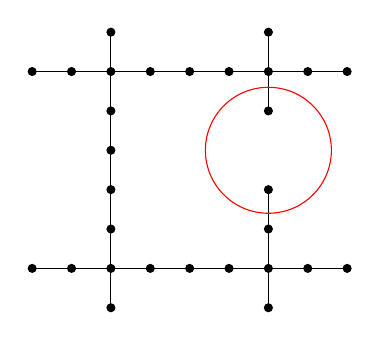
\begin{tikzpicture}
\draw [fill] (7,0.5) circle [radius=0.05];
\draw [fill] (7.5,0.5) circle [radius=0.05];
\draw [fill] (8,0.5) circle [radius=0.05];
\draw [fill] (8.5,0.5) circle [radius=0.05];
\draw [fill] (9,0.5) circle [radius=0.05];
\draw [fill] (9.5,0.5) circle [radius=0.05];
\draw [fill] (10,0.5) circle [radius=0.05];
\draw [fill] (10.5,0.5) circle [radius=0.05];
\draw [fill] (11,0.5) circle [radius=0.05];
\draw [fill] (7,3) circle [radius=0.05];
\draw [fill] (7.5,3) circle [radius=0.05];
\draw [fill] (8,3) circle [radius=0.05];
\draw [fill] (8.5,3) circle [radius=0.05];
\draw [fill] (9,3) circle [radius=0.05];
\draw [fill] (9.5,3) circle [radius=0.05];
\draw [fill] (10,3) circle [radius=0.05];
\draw [fill] (10.5,3) circle [radius=0.05];
\draw [fill] (11,3) circle [radius=0.05];
\draw [fill] (8,0) circle [radius=0.05];
\draw [fill] (8,1) circle [radius=0.05];
\draw [fill] (8,1.5) circle [radius=0.05];
\draw [fill] (8,2) circle [radius=0.05];
\draw [fill] (8,2.5) circle [radius=0.05];
\draw [fill] (8,3.5) circle [radius=0.05];
\draw [fill] (10,0) circle [radius=0.05];
\draw [fill] (10,1) circle [radius=0.05];
\draw [fill] (10,1.5) circle [radius=0.05];
\draw [fill] (10,2.5) circle [radius=0.05];
\draw [fill] (10,3.5) circle [radius=0.05];

\draw (7,0.5) --(11,0.5);
\draw (7,3) --(11,3);
\draw (8,0) --(8,3.5);
\draw (10,0) --(10,1.5);
\draw (10,2.5) --(10,3.5);

\draw [color=red] (10,2) circle[radius=0.8];


\end{tikzpicture}
\caption{$RMST$ for $P$ with a missing road segment indicated by the red circle.}
\label{fig:RMST}
\end{figure}

\begin{figure}
\begin{tikzpicture}
\draw [fill] (7,0.5) circle [radius=0.05];
\draw [fill] (7.5,0.5) circle [radius=0.05];
\draw [fill] (8,0.5) circle [radius=0.05];
\draw [fill] (8.5,0.5) circle [radius=0.05];
\draw [fill] (9,0.5) circle [radius=0.05];
\draw [fill] (9.5,0.5) circle [radius=0.05];
\draw [fill] (10,0.5) circle [radius=0.05];
\draw [fill] (10.5,0.5) circle [radius=0.05];
\draw [fill] (11,0.5) circle [radius=0.05];
\draw [fill] (7,3) circle [radius=0.05];
\draw [fill] (7.5,3) circle [radius=0.05];
\draw [fill] (8,3) circle [radius=0.05];
\draw [fill] (8.5,3) circle [radius=0.05];
\draw [fill] (9,3) circle [radius=0.05];
\draw [fill] (9.5,3) circle [radius=0.05];
\draw [fill] (10,3) circle [radius=0.05];
\draw [fill] (10.5,3) circle [radius=0.05];
\draw [fill] (11,3) circle [radius=0.05];
\draw [fill] (8,0) circle [radius=0.05];
\draw [fill] (8,1) circle [radius=0.05];
\draw [fill] (8,1.5) circle [radius=0.05];
\draw [fill] (8,2) circle [radius=0.05];
\draw [fill] (8,2.5) circle [radius=0.05];
\draw [fill] (8,3.5) circle [radius=0.05];
\draw [fill] (10,0) circle [radius=0.05];
\draw [fill] (10,1) circle [radius=0.05];
\draw [fill] (10,1.5) circle [radius=0.05];
\draw [fill] (10,2.5) circle [radius=0.05];
\draw [fill] (10,3.5) circle [radius=0.05];

\draw (7,0.5) --(11,0.5);
\draw (7,3) --(11,3);
\draw (8,0) --(8,3.5);
\draw (10,0) --(10,3.5);

\draw [fill] (12.5,1) circle [radius=0.05];
\draw [fill] (13,1.5) circle [radius=0.05];
\draw [fill] (13.5,2) circle [radius=0.05];
\draw [fill] (14,2.5) circle [radius=0.05];

\draw (12.5,1) --(13.5,2);
\draw [color=red] (13,2.5) --(14,1.5);
\node at (14,1.3) {$l_1$};
\node at (14,2.8) {$x$};
\node at (13.1,1.8) {$e$};

\draw [fill] (16.5,2.5) circle [radius=0.05];
\draw [fill] (17,2) circle [radius=0.05];
\draw [fill] (17.5,1.5) circle [radius=0.05];
\draw [fill] (18,1) circle [radius=0.05];

\draw (16.5,2.5) --(17.5,1.5);
\draw [color=red] (17,1) --(18,2);
\node at (17,0.8) {$l_1$};
\node at (18.3,1) {$x$};
\node at (17.2,2) {$e$};


\draw [color=red] (10,2) circle[radius=0.8];
\end{tikzpicture}
\caption{Left: $RN_{min}$ road segment in circle is connected. Middle: Slope of $e$ is positive, check if $x$ is above $l_1$. Right: Slope of $e$ is negative, check if $x$ is below $l_1$.}
\label{fig:RNmin}
\end{figure}

\begin{figure}
\begin{tikzpicture}
\draw (7,0.5) --(7.5,0.5);
\draw [color=red](7.5,0.5) --(8,1);
\draw (8,1) --(8,0);
\node at (7.7,1) {$e'$};

\draw [fill] (7,0.5) circle [radius=0.05];
\draw [fill] (7.5,0.5) circle [radius=0.05];
\draw [fill] (8,1) circle [radius=0.05];
\draw [fill] (8,0) circle [radius=0.05];


\draw (13,0.5) --(13.5,0.5);
\draw [color=blue] (13.5,0.5) --(15,0.5);
\draw [color=red](13.5,0.5) --(14,1);
\draw (14,1) --(14,0);
\node at (13.7,1) {$e'$};
\node at (14.2,0.3) {$p$};

\draw [fill] (13,0.5) circle [radius=0.05];
\draw [fill] (13.5,0.5) circle [radius=0.05];
\draw [fill] (14,1) circle [radius=0.05];
\draw [fill] (14,0) circle [radius=0.05];
\draw [color=red, fill] (14,0.5) circle [radius=0.05];

\draw (19,0.5) --(19.5,0.5);
\draw [color=red] (19.5,0.5) --(20,0.5);
\draw (20,1) --(20,0);
\node at (20.2,0.3) {$p$};

\draw [fill] (19,0.5) circle [radius=0.05];
\draw [fill] (19.5,0.5) circle [radius=0.05];
\draw [fill] (20,1) circle [radius=0.05];
\draw [fill] (20,0) circle [radius=0.05];
\draw [color=red, fill] (20,0.5) circle [radius=0.05];

\end{tikzpicture}
\caption{Calculation steps for $RN_{com}$. Left: Edge $e'$ with divergent angle in red. Middle: Blue line intersects at $p$. Right:$e'$ is remove from $RN_{min}$ and new edge $s$ is added to $RN_{com}$ }
\label{fig:RNcom}
\end{figure}

\begin{algorithm}
\caption{Calculate $RMST$ for graph $G(V,E)$}
\begin{algorithmic} 
\STATE $A=\emptyset$
\STATE Sort by increasing $L_1$ distance($E$)
\FORALL{$v \in V$} 
\STATE MAKE-SET($v$)
\ENDFOR
\FORALL{$u$, $v \in E$}
\IF{FIND-SET($u$) $\neq$ FIND-SET($v$)}
\STATE $A=A$ $\cup$ \{($u,v$)\} 
\STATE UNION($u,v$)
\ENDIF
\ENDFOR
\RETURN $A$
\end{algorithmic}
\label{alg:RMSTalg}
\end{algorithm}

\begin{algorithm}
\caption{Calculate $RN_{min}$ for $RMST(V,E)$}
\begin{algorithmic} 
\STATE $A= RMST$
\FORALL{$v\in V$}
\IF{$v$ is a endpoint \textbf{and} adjacentnodes($v$) $\neq$ $\emptyset$}
\STATE $e$ = FIND-SEGMENT($V$)
\REPEAT 
\IF{adjacentnodes[i].direction $=$ $e$.direction }
\STATE $A$.add(new Segment($e$,adjacentnodes[i]))
\ENDIF
\STATE i++
\UNTIL{new segment is added}
\ENDIF
\ENDFOR
\RETURN $A$
\end{algorithmic}
\label{alg:RNminalg}
\end{algorithm}

\begin{algorithm}
\caption{Calculate $RN_{com}$ given $RN_{min})$}
\begin{algorithmic} 
\STATE $A= RN_{min}$
\FORALL{$e \in E$}
\STATE $e'$ = $e$.NEXT-SEGMENT
\IF{$e'$.getSlope $\neq$ $e$.getSlope}
\IF{Direction $e$ intersect with segment $x \in E$}
\IF{Distance between $e$ and $x$ $<$ 0.2f}
\STATE $p$ = new Point at intersection with $x$
\STATE $A=A-e'$
\STATE $s$= new Segment from $e$ to $p$
\STATE $A=A+s$
\ENDIF
\ENDIF
\ENDIF
\ENDFOR
\RETURN $A$
\end{algorithmic}
\label{alg:RNcomalg}
\end{algorithm}


\bibliographystyle{plain}

\begin{thebibliography}{}

\bibitem{k-osssgtsp-56}
J.B. Kruskal.
On the shortest spanning subtree of a graph and the traveling salesman problem.
In \emph{Proceedings of the American Mathematical Society},7: 48-50, 1956.

\bibitem{cghs-rnrop-20}
D. Chen, L.J. Guibas, J. Hershberger, J. Sun.
Road Network Reconstruction for Organizing Paths.
In \emph{Proceedings  of  21st  ACM-SIAM  Symposium  on  Discrete  Algorithms}, 10: 1309-1320, 2010.

\bibitem{a-raoa-02}
S. Albers.
On randomized online scheduling.
In \emph{Proc. 34th ACM Sympos. Theory Comput.}, pages 134--143, 2002.

\bibitem{clrs-ia-01}
T.H. Cormen, C.E. Leiserson, R.L. Rivest and C. Stein.
\emph{Introduction to Algorithms} (2nd edition).
MIT Press, 2001.

\bibitem{m-apca-83}
N. Megiddo.
Applying parallel computation algorithms in the design of serial algorithms.
\emph{J. ACM} 30: 852--865 (1983).

\end{thebibliography}


\begin{itemize}
\item for journals:
      Authors. Title of paper. \emph{Journal Name (italic)} volume: page numbers (year).
      See reference~\cite{m-apca-83}.
\item for conference proceedings:
      Authors. Title of paper. In \emph{Proc. Conference Name and number (italic)}, pages xxx--yyy, year.
      See reference~\cite{a-raoa-02}
\item for books: Authors. \emph{Book title (italic)}. publisher, year.
      See reference~\cite{clrs-ia-01}
\end{itemize}
Note that names of journals and conferences are usually abbreviated. There is a more
or less standard way of doing this (for example, \emph{J. ACM} is stands for \emph{Journal of the ACM},
but how you do it exactly is not so important,
as long as you are consistent and list all the necessary information.






\end{document}

